

%from micro2015template:
\documentclass{sig-alternate}

% Set letter paper size:
\setlength{\paperheight}{11in}
\setlength{\paperwidth}{8.5in}
\usepackage[
  pass,% keep layout unchanged 
  % showframe,% show the layout
]{geometry}

\newcommand{\ignore}[1]{}
\usepackage{fancyhdr}
\usepackage[normalem]{ulem}
\usepackage[hyphens]{url}
\usepackage{hyperref}

% from Yoav's template
\usepackage{color}
\usepackage{xcolor}
\usepackage{graphicx}

%%%%%%%%%%%---SETME-----%%%%%%%%%%%%%
\newcommand{\microsubmissionnumber}{XXX}
%%%%%%%%%%%%%%%%%%%%%%%%%%%%%%%%%%%%

\fancypagestyle{firstpage}{
  \fancyhf{}
\setlength{\headheight}{50pt}
\renewcommand{\headrulewidth}{0pt}
  \fancyhead[C]{\normalsize{MICRO 2016 Submission
      \textbf{\#\microsubmissionnumber} -- Confidential Draft -- Do NOT Distribute!!}} 
  \pagenumbering{arabic}
}  

\usepackage{tabularx}
\usepackage{tabulary}
% more compact + self-contained (with embedded fonts)
\usepackage[T1]{fontenc}
\usepackage[ansinew]{inputenc}
\usepackage{pslatex}
%\usepackage[normalem]{ulem}
%\usepackage{titling}            % control the maketitle
%\setlength{\droptitle}{-3.3em}  % This is your set screw
\usepackage[kerning,spacing]{microtype}
%\microtypecontext{spacing=nonfrench}
\usepackage[caption=false]{subfig}
%\captionsetup{position=top} % put subcations above subfigures
\captionsetup[subfloat]{margin=3pt}

% util
\newcommand{\mypar}[1]{\textbf{#1}\ \ }

% yoav macros
\newcommand{\hide}[1]{}
\setlength{\marginparwidth}{2cm}
%\newcommand{\comment}[1]{\marginpar{\footnotesize #1}}

\newcommand{\comment}[1]{}
%\newcommand{\comment}[1]{\textcolor{red}{[#1]}}

\newcommand{\replace}[2]{
  \textcolor{red}{#1}

  \textcolor{yellow}{#2}
}


\renewcommand{\tilde}[0]{$\sim$}
\newcommand{\us}[0]{$\mu s$}

\newcommand{\speedup}[1]{#1$\times$}
\newcommand{\percent}[1]{#1\% }

%###############################################################################
\title{NeSC: Self Virtualizing Nested Storage Controller}
%###############################################################################

\begin{document}
\maketitle
\thispagestyle{firstpage}
\pagestyle{plain}


\author{
  {\rm
  Yonatan Gottesman$^{\dagger}$
  Yoav Etsion$^{\dagger}$}\\[0mm]
  $^\dagger$Technion---Israel Institute of Technology
}

%% %###############################################################################
%% \begin{document}
%% \date{}
%% \maketitle


%###############################################################################
% abstract
%###############################################################################
\begin{abstract}
The emergence of high-speed, multi GB/s storage devices has shifted the performance bottleneck of storage virtualization to the software layers of the hypervisor. The hypervisor overheads can be avoided by allowing the virtual machine (VM) to directly access the storage device (a method known as direct device assignment), but this method voids all protection guarantees provided by  filesystem permissions, since the device has no notion of client isolation.
Recently, following the introduction of 10Gbs and higher networking interfaces, the PCI-SIG was extended to include the SR-IOV specification for self-virtualizing devices, which allows a single physical device to present multiple virtual interfaces on the PCIe interconnect. Using SR-IOV, a hypervisor can directly assign a virtual PCIe device interface to each of its VMs. However, as networking interfaces simply multiplex packets sent from/to different clients, the specification does not dictate the semantics of a virtual storage device and how to maintain data isolation in a self virtualizing device.



  In this paper we present the self-virtualizing, nested storage controller (NeSC) architecture, which includes a filesystem-agnostic protection mechanism that enables the physical device to export files as virtual PCIe storage devices. The protection mechanism maps file offsets to physical blocks and thereby offloads the hypervisor's storage layer functionality to hardware.
  Using NeSC, a hypervisor can securely expose its files as virtual PCIe devices and directly assign them to VMs.
  We have prototyped a 1GB/s NeSC controller using a Virtex-7 FPGA development board connected to the PCIe interconnect. 
  Our evaluation of NeSC on a real system shows that NeSC virtual devices enable VMs to access to their data with near-native performance (in terms of both throughput and latency).
\end{abstract}

\replace{
  this is the original paragraph.
}{
  this is the new paragraph.
}


%###############################################################################
%%%%%%%%%%%%%%%%%%%%%%%%%%%%%%%%%%%%%%%%%%%%%%%%%%%%%%%%%%%%%%%%%%%%%%%%
\section{Introduction}
\label{sec:intro}

%%%%%%%%%%%%%%%%%%%%%%%%%%%%%%%%%%%%%%%%%%%%%%%%%%%%%%%%%%%%%%%%%%%%%%%%
%%%%%%%%%%%%%%%%%%%%%%%%%%%%%%
% moved here from motivation section.
%%%%%%%%%%%%%%%%%%%%%%%%%%%%%%
\begin{figure*}[ht!]
  \centering
    \subfloat[Emulation ]{
      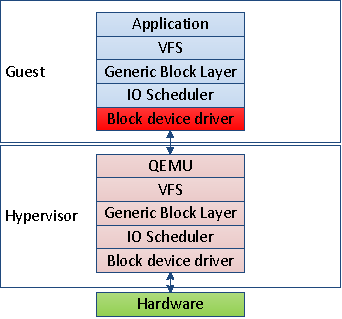
\includegraphics[width=0.3\textwidth]{figs/emulation.pdf}
      \label{fig:storage:emulation}
    }
    \hfill
    \subfloat[virtio]{
      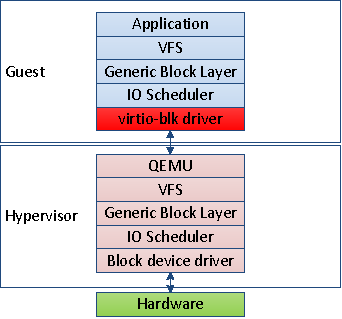
\includegraphics[width=0.3\textwidth]{figs/virtio.pdf}
      \label{fig:storage:virtio}
    }
    \hfill
    \subfloat[Direct-IO]{
      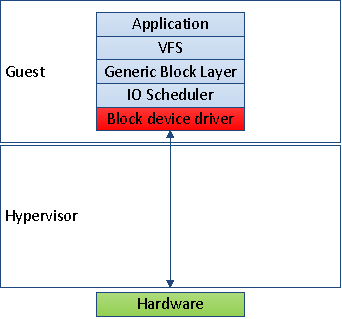
\includegraphics[width=0.3\textwidth]{figs/direct.pdf}
      \label{fig:storage:direct}
    }
    \caption{IO Virtualization techniques.
      \label{fig:storage}}
    
\end{figure*}
%%%%%%%%%%%%%%%%%%%%%%%%%%%%%%

The prevalence of machine consolidation through the use of virtual machines (VMs) necessitates improvements in VM performance. On the architecture side, major processor vendors have introduced virtualization extensions to their instruction set architectures~\cite{popek1974formal,intel,armv8}.
The emergence of high-speed networking interfaces also requires that VMs be granted direct access to  physical devices, thereby eliminating the costly, software-based hypervisor device multiplexing.

Enabling untrusted VMs to directly access physical devices, however, compromises system security.
To overcome the fundamental security issue, the PCIe specification was extended to support self-virtualizing devices through the Single-Root I/O Virtualization (SR-IOV) interface~\cite{pcisigiov}).
This method enables a physical device (\emph{physical function} in SR-IOV parlance) to dynamically create virtual instances (\emph{virtual functions}). Each virtual instance receives a separate address on the PCIe interconnect and can, therefore, be exclusively assigned to, and accessed by, a specific VM. This method thereby distinguishes between the physical device, managed by the hypervisor, and its virtual instances used by the VMs.
%
Importantly, it is up to the physical device to interleave and execute requests issued to the virtual devices.

Self-virtualizing devices thus delegate the task of multiplexing VM requests from the software hypervisor to the device itself.
The multiplexing policy, however, depends on the inherent semantics of the underlying device and must, naturally, isolate request streams sent by individual virtual devices (that represent client VMs).
For some devices, such as networking interfaces, the physical device can simply interleave the packets sent by its virtual instances (while protecting the shared link state~\cite{smolyar15sriovsec}).
%performance of direct assignment with flexibility of emulation
%
However, enforcing isolation is nontrivial when dealing with storage controllers/devices, which typically store a filesystem structure maintained by the hypervisor. The physical storage controller must therefore enforce the access permissions imposed by the filesystem it hosts.
%
%SHARON?
The introduction of next-generation, commercial PCIe SSDs that deliver multi-GB/s bandwidth~\cite{intel-ssd,seagate16ssd}) emphasizes the need for self-virtualizing storage technology.

In this paper we present NeSC, a self-virtualizing nested storage controller that enables hypervisors to expose files and persistent objects\footnotemark (or sets thereof) as virtual block devices that can be directly assigned to VMs.
\footnotetext{We use the terms files and objects interchangeably in this paper.}

  NeSC implements the SR-IOV specification, which allows it to expose itself through multiple dynamically allocated PCIe addresses. This enables NeSC to present itself as multiple virtual storage devices (through the distinct PCIe addresses) that are directly assigned to VMs. By multiplexing the requests sent by the VMs to each virtual device, NeSC can enforce the access permissions set by the hypervisor and prevent VMs from  accessing stored data for which they have no access permissions.

NeSC enforces isolation by associating each virtual NeSC device with a table that maps offsets in the virtual device to blocks on the physical device. This process follows the way filesystems map file offsets to disk blocks.
%
VMs view virtual NeSC instances as regular PCIe storage controllers (block devices). Whenever the hypervisor wishes to grant a VM direct access to a file, it queries the filesystem for the file's logical-to-physical mapping and instantiates a virtual NeSC instance associated with the resulting mapping table.
%
Each access by a VM to its virtual NeSC instance is then transparently mapped by NeSC to a physical disk block using the mapping table associated with the virtual device (e.g., the first block on the virtual device maps to offset zero in the mapped file).

We evaluate the performance benefits of NeSC using a real working prototype implemented on a Xilinx VC707 FPGA development board. Our evaluation shows that our NeSC prototype, which provides 800MB/s read bandwidth and almost 1GB/s write bandwidth, delivers \speedup{2.5} and \speedup{3} better read and write bandwidth, respectively, compared to a paravirtualized \emph{virtio}~\cite{russell2008virtio} storage controller (the de facto standard for virtualizing storage in Linux hypervisors), and \speedup{4} and \speedup{6} better read and write bandwidth, respectively, compared to an emulated storage controller.
We further show that these performance benefits are limited only by the bandwidth provided by our academic protoype. We expect that NeSC will greatly benefit commercial PCIe SSDs capable of delivering multi-GB/s of bandwidth.



Although this paper focuses on the performance benefits that NeSC provides for VMs, it is important to note that NeSC also provides secure and direct storage access for accelerators connected to the PCIe interconnet (e.g., GPGPUs, FPGAs). As virtual NeSC instances are directly accessible on the PCIe interconnect, they can be accessed directly by other PCIe devices (using direct device DMA), thereby removing the CPU from the accelerator-storage communication path.

In this paper we make the following contributions:
\begin{itemize}
\item
 We introduce NeSC, a self-virtualizing, nested storage controller that offloads file mapping and permission check operations to hardware and provides VMs with direct and secure storage access without hypervisor mediation.

\item
  We propose a hardware implementation for NeSC, which is prototyped using a Xilinx VC707 (Virtex-7) FPGA development board.

\item
  We evaluate the benefit of self-virtualizing storage using microbenchmarks and complete applications. Our evaluation shows that the NeSC prototype delivers \speedup{2.5} and \speedup{3} better read and write bandwidth, respectively, than state-of-the-art software virtual storage.
  
\end{itemize}


The rest of this paper is organized as follows:
Section~\ref{sec:motiv} discusses the performance overheads of storage virtualization, and  Section~\ref{sec:related} discusses related work.
We present the NeSC system design in Section~\ref{sec:design} and its architecture in Section~\ref{sec:arch}. We then present our evaluation methodology in Section~\ref{sec:methodology}, the evaluation in Section~\ref{sec:eval}, and conclude in Section~\ref{sec:conclusions}.




%%%%%%%%%%%%%%%%%%%%%%%%%%%%%%%%%%%%%%%%%%%%%%%%%%%%%%%%%%%%%%%%%%%%%%%%
\section{On the performance overheads of storage virtualization}
\label{sec:motiv}
%%%%%%%%%%%%%%%%%%%%%%%%%%%%%%%%%%%%%%%%%%%%%%%%%%%%%%%%%%%%%%%%%%%%%%%%

Hypervisors virtualize local storage resources by mapping guest storage devices onto files in their local filesystem, in a method commonly referred to as a nested filesystem~\cite{le12nested}. As a result, they replicate the guest operating system's (OS) software layers that abstract and secure the storage devices. Notably, these software layers have been shown to present a performance bottleneck even when not replicated~\cite{yu14swoverheads}, due to the rapid increase in storage device bandwidth ~\cite{intel-ssd,seagate16ssd}.
%
Moreover, further performance degradation is caused by the method by which hypervisors virtualize storage devices and the resulting communication overheads between the guest OS and the underlying hypervisor.
Consequently, the storage system is becoming a major bottleneck in modern virtualized environments.
%
In this section we examine the sources of these overheads and outline how they can be mediated using a self-virtualizing storage device.

% software layers
Prevalent storage devices present the software stack with a raw array of logical block addresses (LBA), and it is up to the OS to provide a flexible method to partition the storage resources into logical objects, or files. In addition, the OS must enforce security policies to prevent applications from operating on data they are not allowed to operate on.
%
The main software layer that provides these functionalities is the filesystem, which combines both allocation and mapping strategies to construct logical objects and map them to physical blocks (for brevity, we focus the discussion on these two functionalities and ignore the plethora of other goals set by different filesystems). In addition, the filesystem layer also maintains protection and access permissions. Besides the filesystem, another common layer is the block layer, which caches disk blocks and abstracts the subtleties of different storage devices from the filesystem layer.

When an application accesses a file, the OS uses the filesystem layer to check the access permissions and map the file offset to an LBA on the storage device. It then accesses its block layer, which retrieves the block either from its caches or from the physical device. In a VM, this process is replicated since the storage device viewed by the guest OS is actually a virtual device that is mapped by the hypervisor to a file on the host's storage system. Consequently, the hypervisor invokes its own filesystem and block layers to retrieve the data to the guest OS. 

% virtualization method
Figure~\ref{fig:storage} illustrates the three most common methods by which hypervisors virtualize storage devices:

\begin{enumerate}
\item
  \emph{Full device emulation}~\cite{sugerman2001virtualizing} (Figure~\ref{fig:storage:emulation})\quad 
  In this method, the host emulates a known device that the guest already has a driver for. The host traps device accesses by the VM and converts them to operations on real hardware. The emulated device is represented as a file on the host filesystem, and whenever the guest tries to access a virtual LBA on the device, the host converts the virtual LBA to an offset in the file.

\item
  \emph{Paravirtualization}~\cite{barham2003xen,russell2008virtio} (Figure~\ref{fig:storage:virtio})\quad
  This method, commonly referred to as virtio after its Linux implementation, eliminates the need for the hypervisor to emulate a complete physical device and enables the guest VM to directly request a virtual LBA from the hypervisor, thereby improving performance. This is the most common storage virtualization method used in modern hypervisors.

\item
  \emph{Direct device assignment}~\cite{raj2007high} (Figure~\ref{fig:storage:direct})\quad
  This method allows the guest VM to directly interact with the physical device without hypervisor mediation. Consequently, it delivers the best storage performance to the VM. However, since storage devices do not enforce isolation among clients, it does not allow multiple VMs to share a physical device.
\end{enumerate}

%%%%%%%%%%%%%%%%%%%%%%%%%%%%%%
\begin{figure}[t]
  \centering
  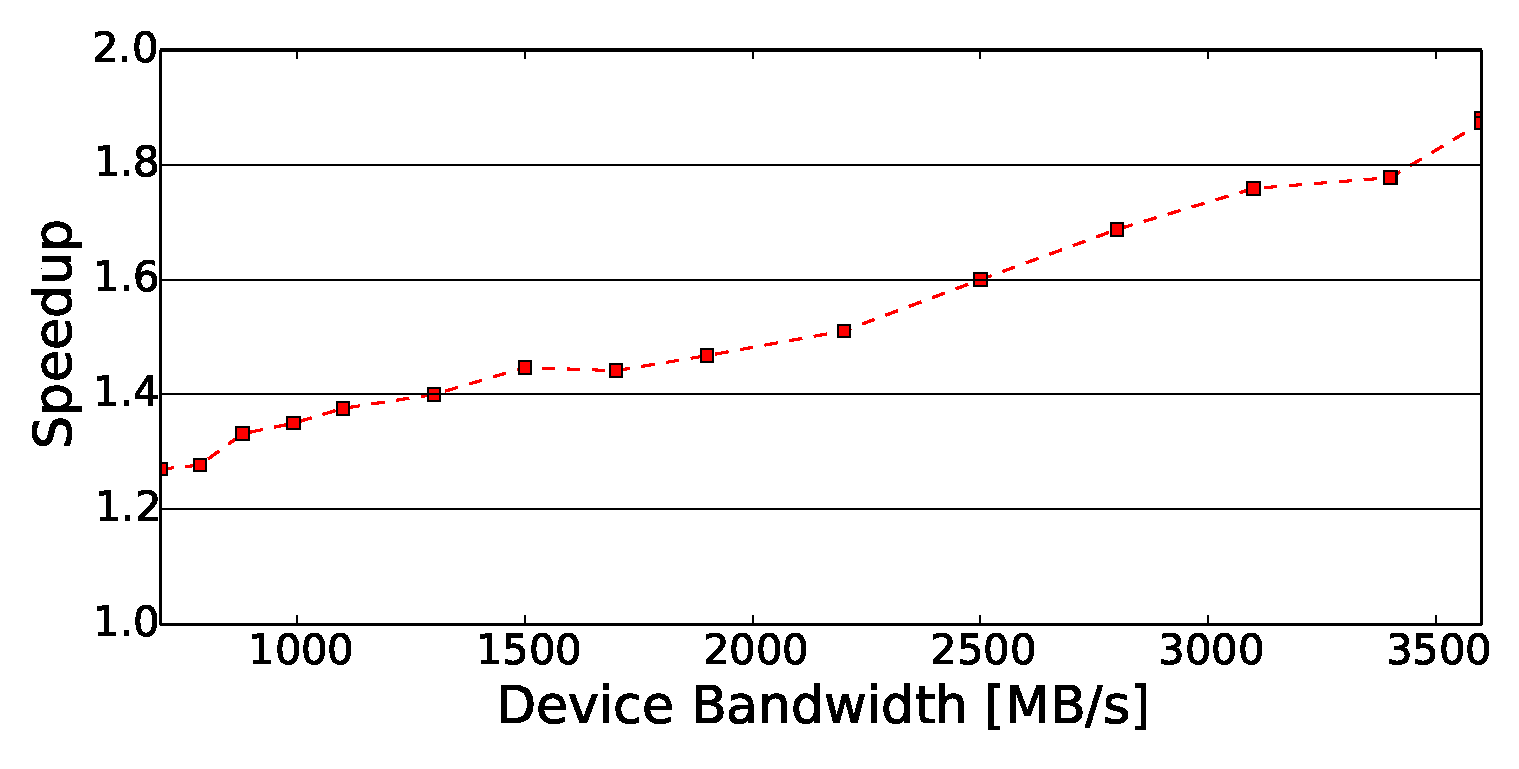
\includegraphics[width=\columnwidth]{figs/motivation.pdf}
  \caption{The performance benefit of direct device assignment over virtio for high-speed storage devices. Fast devices were emulated using an in-memory disk (ramdisk) whose bandwidth, due to the overheads of the software layers, peaks at 3.6GB/s.
    \label{fig:directperf}}
  \end{figure}
%%%%%%%%%%%%%%%%%%%%%%%%%%%%%%

% quantify the overheads
Figure~\ref{fig:directperf} quantifies the potential bandwidth speedup of direct device assignment over the common virtio interface for high-speed storage devices. We have emulated such devices by throttling the bandwidth of an in-memory storage device (ramdisk). Notably, due to OS overhead incurred by its software layers, the ramdisk bandwidth peaks at 3.6GB/s.

The figure shows the raw write speedups obtained using direct device assignment over virtio for different device speeds, as observed by a guest VM application.
Notably, we see that compared to the state-of-the-art virtio method, direct device assignment roughly doubles the storage bandwidth provided to virtual machines for modern, multi GB/s storage devices.
The reason for these speedups is that as device bandwidth increases, the  software overheads associated with virtualizing a storage device become a performance bottleneck.
Using the direct device assignment method eliminates both the virtualization overheads as well as the overheads incurred by the replication of the software layers in the hypervisor and the guest OS.

% we need NeSC
The potential performance benefits of direct device assignment motivate the incorporation of protection and isolation facilities into the storage device. These facilities will enable multiple guest VMs to share a directly accessed physical device without compromising data protection.

%%%%%%%%%%%%%%%%%%%%%%%%%%%%%%
\begin{figure}[t]
  \centering
  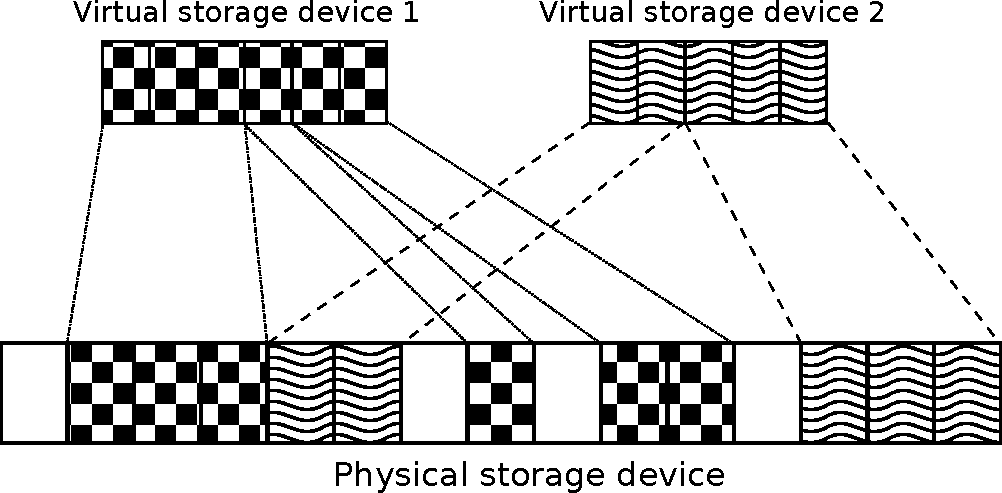
\includegraphics[width=\columnwidth]{figs/nesc-overview.pdf}
  \caption{Exporting files as virtual devices using NeSC.\label{fig:nesc_outline}}  
\end{figure}
%%%%%%%%%%%%%%%%%%%%%%%%%%%%%%

This paper presents the nested storage controller (NeSC), which enables multiple VMs to concurrently access files on the host's filesystem without compromising storage security (when NeSC manages a single disk, it can be viewed simply as a PCIe SSD).
Figure~\ref{fig:nesc_outline} illustrates how NeSC provides VMs with secure access to a shared physical device.
NeSC leverages the SR-IOV features of the PCIe gen3~\cite{pcisigiov} to export host files as multiple virtual devices on the PCIe address space. Each virtual device is associated with a collection of non-contiguous blocks on the physical device, which represent a file, and is \comment{sharon v3. I think we are ok here} prevented from accessing other blocks. VMs can therefore directly access the virtual device and bypass the virtualization protocol and hypervisor software (notably, NeSC is compatible with the modern NVMe standard~\cite{nvme}).
The rest of this paper describes the design, architecture, and evaluation of NeSC.




%% Storage devices inherently maintain state and do not enforce isolation, requiring software to do so.
%% - client requests the OS to fetch a file/object. OS uses filesystem to logically partition storage to multiple files/objects
%% - Storage devices were traditionally slow, so software overhead was not an issue
%% - Prevalent PCIe and NVMe storage devices are much faster, so having the software on the critical path has become an issue
%% - We need direct device access to ameliorate the overheads of virtualization, but that requires that devices transparently enforce isolation between clients
%% - need to maintain the flexibility provided by the filesystem abstraction%


%% \cite{nested-filesystems}


%% % discuss this vs. partition-based direct accesses
%% filesystems provide management flexibility


%% 1. VMs need direct access to files (image file, data files)
%% - esp. in the context of emerging memory technologies \cite{huang2015unified}.
%% - files/object are a dynamically flexible storage abstraction
%% - easy to change content, size
%% - easy to move between machines (as opposed to partitions)

%% 2. hardware has no notion of files/objects, so it provides no isolation guarantees
%% - VM can access an entire disk/partition, not part thereof.
%% - object-level isolation must be maintained at the software level, with substantial overheads
%% - *Figure* depicted storage virtualization using existing designs (emulation, paravirt, direct device I/O)

%% 3. we introduce hardware-based object virtualization
%% - hardware enforces isolation at wire speed (gets software off the critical path)
%% - maintains flexibility and generality of traditional filesystems.


%% - SR-IOV alone does not provide what we need
%%   - SR-IOV allow to dynamically create logical devices.
%%   - it does not say anything about what is the meaning of the ``logical device'' (e.g., the relation between a physical NIC and a logical NIC is different than the relation between a physical storage device and a logical one)

%% Each vdisk is a represented as a file so easy to migrate  
%% asd


%% discuss the potential performance benefits due to nested filesystems \cite{le12nested}

%% %%%%%%%%%%%%%%%%%%%%%%%%%%%%%%%%%%%%%%%%%%%%%%%%%%
%% \subsection{Supporting direct accelerators-storage accesses}
%% %%%%%%%%%%%%%%%%%%%%%%%%%%%%%%%%%%%%%%%%%%%%%%%%%%
%% save power and not need to interfere with CPU 

%%%%%%%%%%%%%%%%%%%%%%%%%%%%%%%%%%%%%%%%%%%%%%%%%%
\section{Related Work}
\label{sec:related}
%%%%%%%%%%%%%%%%%%%%%%%%%%%%%%%%%%%%%%%%%%%%%%%%%%

NeSC examines the design of the hardware/software storage stack for modern, high-speed, self-virtualizing storage devices. In this section we examine related research efforts.

The Moneta~\cite{caulfield10moneta} and Moneta-D~\cite{caulfield12moneta-d} projects both try to optimize the I/O stack by introducing new hardware/software interfaces.
The Moneta project introduces a storage array architecture for high-speed non-volatile memories. Moneta-D extends the design to allow applications
to directly access storage by introducing per-block capabilities~\cite{levy1984capability}. When an application directly accesses the storage, permission checks are done by the hardware to preserve protection policies dictated by the OS.
The design, however, requires applications to use a user space library to map a file offsets to the physical blocks on the device.
In contrast, NeSC enforces file protection by delegating file mapping to the device level rather than to the application level.

Willow~\cite{seshadri2014willow} examines offloading computation to small storage processing units (SPU) that reside on the SSD. The SPUs run a small OS (SPU-OS) that enforces data protection. Willow implements a custom software protocol that maintains file mapping coherence between the main OS and the SPU-OS instances.

NVMe~\cite{nvme} is a new protocol for accessing high-speed storage devices. Typically implemented over PCIe, NVMe defines an abstract concept of \emph{address spaces} through which applications and VMs can access subsets of the target storage device. The protocol, however, does not specify how address spaces are defined, how they are maintained, and what they represent. 
NeSC therefore complements the abstract NVMe address spaces and enables the protocol to support protected, self-virtualizing storage devices.

Finally, FlashMap~\cite{huang2015unified} provides a unified translation layer for main memory and SSDs, which enables applications to map files to their memory address space. Specifically, FlashMap unifies three orthogonal translation layers used in such scenarios: the page tables, the OS file mapping, and the flash translation layer.
FlashMap, however, only supports memory-mapped SSD content, and it does not address how the unified translation would support virtualized environments.

In summary, NeSC's self-virtualizing design is unique in that it delegates all protection checks and filesystem mappings to the hardware. Furthermore, its  filesystem-agnostic design preserves the hypervisor's flexibility to select and manage the host filesystem.




%%%%%%%%%%%%%%%%%%%%%%%%%%%%%%%%%%%%%%%%%%%%%%%%%%%%%%%%%%%%%%%%%%%%%%%%
\section{Design}
\label{sec:design}
%%%%%%%%%%%%%%%%%%%%%%%%%%%%%%%%%%%%%%%%%%%%%%%%%%%%%%%%%%%%%%%%%%%%%%%%

In this section we overview the NeSC design principles and basic functionality. 

%%%%%%%%%%%%%%%%%%%%%%%%%%%%%%%%%%%%%%%%%%%%%%%%%%
\subsection{The NeSC interface}
%%%%%%%%%%%%%%%%%%%%%%%%%%%%%%%%%%%%%%%%%%%%%%%%%%
NeSC implements the SR-IOV standard \cite{pcisigiov}, which allows an I/O device to be shared by multiple VMs.
An SR-IOV device can present itself as multiple standard PCIe devices. A single \emph{physical function} (PF) represents the main devices with all its features. Additionally, the device may dynamically expose multiple {virtual functions} (VFs), which typically present to clients (e.g., VMs, accelerators) a subset of features supported by the main device. Importantly, each VF has a unique PCIe address and can receive direct I/O requests from its associated client without hypervisor or OS intervention.
%
Since both the PF and the VFs effectively represent different facets of a single physical device, which multiplexes and processes the communication of all the clients with the different facets.
%
It is thus up to the physical device to determine the behavior of the device exported as the PF and that of a virtual device exposed as a VF.

%%%%%%%%%%%%%%%%%%%%%%%%%%%%%%%%%%%%%%%%%%%%%%%%%%
\subsubsection*{The physical function}
%%%%%%%%%%%%%%%%%%%%%%%%%%%%%%%%%%%%%%%%%%%%%%%%%%
The NeSC PF exports a full-featured PCIe storage controller. It is mapped only to the hypervisor address space and allows it to fully manage the physical  device.
The hypervisor uses the PF interface to
(1) manage the underlying NeSC storage and thereby its filesystem;
and (2) manage the NeSC virtual devices by controlling the creation and deletion of VFs and the subsets of storage they are allowed to access.

%%%%%%%%%%%%%%%%%%%%%%%%%%%%%%%%%%%%%%%%%%%%%%%%%%
\subsubsection*{Virtual functions}
%%%%%%%%%%%%%%%%%%%%%%%%%%%%%%%%%%%%%%%%%%%%%%%%%%
Each NeSC VF is viewed by the system as a PCIe device that provides a complete block device interface. A VF can thus be mapped to a VM's address space and viewed by it as a fully fledged storage device, which can be programmed by the VM's driver to issue read/write commands to the storage device. Technically, the only difference between the PF and VF interface is that a VF is not allowed to create nested VFs (although, in principle, such a mechanism can be implemented to support nested virtualization).

The PF and VF differ semantically in that VFs can only access the subset of the storage they are associated with. When a VM accesses a VF, all of its read/write block requests are translated to the subset of blocks assigned to that VM as described below.

%%%%%%%%%%%%%%%%%%%%%%%%%%%%%%%%%%%%%%%%%%%%%%%%%%
\subsection{Virtual-to-physical block mapping}
%%%%%%%%%%%%%%%%%%%%%%%%%%%%%%%%%%%%%%%%%%%%%%%%%%

Decoupling the PF from the VFs enables the hypervisor to logically manage the physical device with its own filesystem, and expose files (or collections thereof) to client VMs as raw virtual devices through VFs (as illustrated in Figure~\ref{fig:nesc_outline}). Each VF is thus associated with a mapping table that translates client requests to physical blocks. Specifically, since client VMs view VFs as regular block devices, they send requests pertaining to LBAs on the virtual device. NeSC refers to client LBAs as virtual LBAs (vLBA), to host LBAs as physical LBAs (pBLA), and the translation process is referred to as a vLBA-to-pLBA translation.

The vLBA-to-pLBA mapping is performed using per-VF mapping tables. The mapping tables are designed as \emph{extent trees}, a method inspired by modern UNIX filesystems.
%
Traditionally, UNIX-derived filesystems used per-file direct and indirect  block mapping tables to map offsets in a file to their corresponding data block. But tracking individual blocks incurs large spatial and latency overheads when dealing with large files. Modern UNIX filesystems (e.g., ext4~\cite{mathur07ext4}, btrfs~\cite{rodeh13btrfs}, xfs~\cite{sweeney96xfs}) therefore group contiguous physical blocks into \emph{extents} and construct extent trees, which consist of variants of B-trees~\cite{comer79btree}, to spatially map offsets in the device to extents.
Each file is associated with an extent tree (pointed to by the file's \emph{inode}) that maps file offsets to physical blocks.

The key benefit of extent trees is that their depth is not fixed but rather depends on the mapping itself. In ext4, for example, a 100MB file can be allocated using a single extent, thereby obviating the need to create the indirect mappings for each individual block. Extents thus improve performance and also reduce management overheads.

%%%%%%%%%%%%%%%%%%%%%%%%%%%%%%%%%%%%%%%%%%%%%%%%%%
\begin{figure*}[t]
  \centering
      \subfloat[Extent tree ]{
        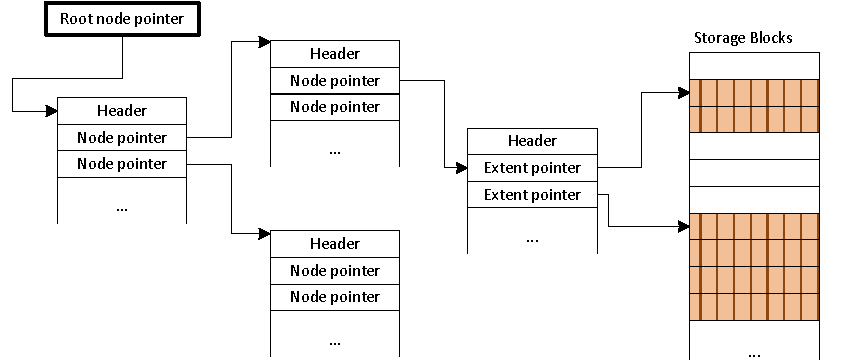
\includegraphics[width=0.7\textwidth]{figs/Ext4_extents.pdf}
        \label{fig:extent_tree}
      }
%      \hfill
      \subfloat[An extent/node pointer entry.]{
%      \centering
      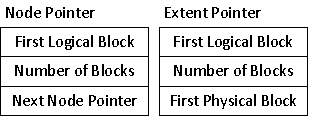
\includegraphics[width=0.3\textwidth]{figs/extent_feilds.pdf}
      \label{fig:extent_fields}
    }
%    \hfill

      \caption{An extent tree used for address translations.\label{fig:extent}}

\end{figure*}
%%%%%%%%%%%%%%%%%%%%%%%%%%%%%%%%%%%%%%%%%%%%%%%%%%

Figure~\ref{fig:extent_tree} illustrates the NeSC VF extent tree (which resembles the ext4 extent tree format). Each node in the tree comprises either a group of node pointers, which point to the next level of nodes, or a group of extent pointers, which are the tree leaves that point to the physical location of the extents. The header of each node indicates whether it contains node indices or extent pointers.

%% %%%%%%%%%%%%%%%%%%%%
%% \begin{figure}[t]
%% %  \vspace*{-1.5ex}
%%   \centering
%%     \subfloat[An extent pointer entry.]{
%% %      \centering
%%       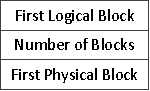
\includegraphics[width=0.2\textwidth]{figs/extent.pdf}
%%       \label{fig:extent}
%%     }
%% %    \hfill
%%     \subfloat[A node pointer entry]{
%% %     \centering
%%       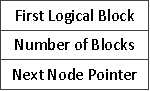
\includegraphics[width=0.2\textwidth]{figs/extent_index.pdf}
%%       \label{fig:extent-index}
%%     }
%%     \caption{Content of extent pointer and node pointer entries.\label{fig:extent_struct}
%%       \comment{TO YOAV: How should this figure look like? its just the fields in a struct so maybe we can just not use an image.  I dont mind using ``node/extent entry'' if its easier to explain but in ext4 its extent-index and extent.  }}
%% \end{figure}
%%%%%%%%%%%%%%%%%%%%

Figure~\ref{fig:extent_fields} illustrates the content of the entries in each type of node in the extent tree. Each \emph{extent pointer} entry consists of the first logical block it represents, a pointer to the first physical block of its extent, and the size of the extent. Each \emph{node pointer} entry comprises the first logical block it represents, the number of (non contiguous) logical blocks it covers, and a pointer to its array of child nodes.

Each  NeSC's VF is associated with an extent tree, which is stored in host memory, and the NeSC architecture (described in Section~\ref{sec:arch}) stores the pointer to the root of each VF's extent tree. Whenever a VF is accessed, its extent tree is traversed using DMA accesses from the device to host memory. To mitigate the DMA latency, extents are cached on the NeSC device (more on this in Section~\ref{sec:arch}).

Importantly, this use of software-defined, hardware-traversed per-VF extent trees eliminates the need to enforce protection and isolation in the hypervisor software layers, as discussed in Section~\ref{sec:motiv}. Instead, this task is offloaded to hardware and thereby mitigates one of the key performance bottlenecks of virtualized storage~\cite{le12nested}.

The per-VF extent tree model also enables the hypervisor to decouple the virtual device's size from its physical layout. This allows the hypervisor to initialize virtual devices whose logical size is larger than their allocated physical space, and to allocate further physical space when needed. This enables the hypervisor to maintain a compact physical representation of the stored data.

Finally, the NeSC design also enables multiple VFs to share an extent tree and thereby files. Nevertheless, NeSC only guarantees the consistency of the extent tree for shared files; it is up to the client VMs to address data synchronization and consistency issues.

%%%%%%%%%%%%%%%%%%%%%%%%%%%%%%%%%%%%%%%%%%%%%%%%%%%%%%%%%%%%%%%%%%%%%%
\subsection{Operational flow}
%%%%%%%%%%%%%%%%%%%%%%%%%%%%%%%%%%%%%%%%%%%%%%%%%%%%%%%%%%%%%%%%%%%%%%

%%%%%%%%%%%%%%%%%%%%%%%%%%%%%%%%%%%%%%%%%%%%%%%%%%
\subsubsection*{Creating a new virtual disk}
%%%%%%%%%%%%%%%%%%%%%%%%%%%%%%%%%%%%%%%%%%%%%%%%%%

When creating a new virtual device, the hypervisor first creates the extent tree that will map the virtual device to physical blocks. Since most modern filesystems use extent trees to map files to their physical layout, this stage typically consists of translating the filesystem's own per-file extent tree to the NeSC tree format. The hypervisor does not fully preallocate all the physical blocks needed for the new virtual device (i.e., lazy allocation). 

The hypervisor then creates a new NeSC VF through the PF. It initializes the VF configuration registers (e.g., the size of the virtual device), writes the extent tree to non-swappable memory and sets the VF's base extent tree configuration register to point to the in-memory extent tree.

Following the two previous steps, the VF is ready and the virtual device is configured. The hypervisor then connects the VM to the new virtual machine, either by executing a new machine or by notifying an existing machine that a new device is available for its use (virtual device hotplug).

%%%%%%%%%%%%%%%%%%%%
\begin{figure*}[t]

  \vspace*{-1.5ex}
  \centering
  \subfloat[Read Flow ]{
    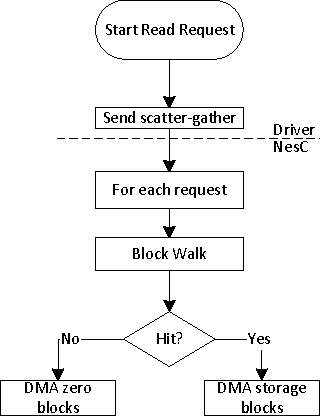
\includegraphics[width=0.85\columnwidth]{figs/read_flow.pdf}
 %   \caption{Read Flow}
    \label{fig:read_flow}
  }
  \hfill
  %% \vspace*{-1.5ex}
  \subfloat[Write Flow ]{
    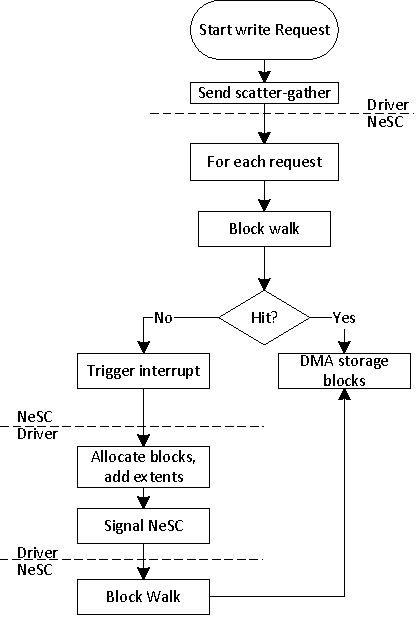
\includegraphics[width=0.85\columnwidth]{figs/write_flow.pdf}
%    \caption{Write Flow}
    \label{fig:write_flow}
  }
  \caption{Read and write flow in NeSC.\label{fig:flow}}
\end{figure*}
%%%%%%%%%%%%%%%%%%%%

%%%%%%%%%%%%%%%%%%%%%%%%%%%%%%%%%%%%%%%%%%%%%%%%%%
\subsubsection*{Read flow}
%%%%%%%%%%%%%%%%%%%%%%%%%%%%%%%%%%%%%%%%%%%%%%%%%%
The read flow is depicted in Figure~\ref{fig:read_flow}. The VM's NeSC block driver is attached to the VF and can issue read requests to the device. Large requests are broken down by the driver to scatter-gather lists of smaller chunks. Our NeSC implementation operates at 1KB block granularity (which is, for example, the smallest block size supported by ext4), so the chunks sent by the block driver are broken down by NeSC to 1KB blocks.

The device then translates each 1024 byte request address through the extent tree mappings of that virtual function and creates a new queue of physical requests to read from physical storage and DMA back to the host memory.

According to the POSIX standard, reads from unmapped areas inside a file (holes in the file) should return zero. Therefore, if the destination vLBA is not mapped in the extent tree, NeSC transparently DMAs zeros to the destination buffer in host memory.

%%%%%%%%%%%%%%%%%%%%%%%%%%%%%%%%%%%%%%%%%%%%%%%%%%
\subsubsection*{Write flow}
%%%%%%%%%%%%%%%%%%%%%%%%%%%%%%%%%%%%%%%%%%%%%%%%%%

The write flow is shown in Figure~\ref{fig:write_flow}. Just like read requests, write requests are broken down by NeSC to 1KB chunks.

For each chunk, the device tries to perform vLBA-to-pLBA mapping using the VF's extent tree. If the translation succeeds, the data is written to the persistent physical storage.
However, lazy allocation may cause  the translation to fail, in which case new physical blocks should be allocated to the VF. Because the VF represents a file in the hypervisor's filesystem, the allocation must be delegated to the hypervisor. NeSC implements this by sending an allocation request interrupt to the hypervisor and stalling the VF until the hypervisor allocates more physical storage.
%
Upon receiving the interrupt, the hypervisor allocates more physical blocks for the the file, updates the VF's extent tree, and signals completion to the NeSC device. NeSC then unstalls the VF's request by restarting the extent tree lookup, which is now guaranteed to succeed. If, however, the hypervisor cannot allocate more space for the VF (not shown in Figure~\ref{fig:write_flow}) due to a lack of physical storage or exhausted storage quotas, it signals an error to the PF which, in turn, triggers the VF to send a write failure interrupt to the requesting VM (we note that it is possible to optimize this process by delegating the interrupt directly to the VM~\cite{gordon12eli}).

%%%%%%%%%%%%%%%%%%%%%%%%%%%%%%%%%%%%%%%%%%%%%%%%%%%%%%%%%%%%%%%%%%%%%%
\subsection{Other design issues}
%%%%%%%%%%%%%%%%%%%%%%%%%%%%%%%%%%%%%%%%%%%%%%%%%%%%%%%%%%%%%%%%%%%%%%

%%%%%%%%%%%%%%%%%%%%%%%%%%%%%%%%%%%%%%%%%%%%%%%%%%
\subsubsection*{Nested filesystems}
%%%%%%%%%%%%%%%%%%%%%%%%%%%%%%%%%%%%%%%%%%%%%%%%%%
A client VM will often manage its own filesystem inside its nested storage device. Given that a virtual device is stored as a file in the hypervisor's filesystem, this use case is commonly referred to as a nested filesystem.

Modern filesystems frequently use journaling for improved fault tolerance. This causes a well-known inefficiency in nested filesystems known as nested journaling~\cite{le12nested}. The inefficiency is caused as both the internal and external filesystems redundantly log the internal filesystem's data and meta-data updates. The common solution to this inefficiency is to tune the hypervisor's filesystem to only log meta-data changes for the file at hand and let the VM handle its internal filesystem's data integrity independently.

NeSC naturally lends itself to this common solution. Since NeSC VM clients directly access their data, the hypervisor's filesystem is not aware of the internal filesystem updates, whose integrity it handled by the VM, and only tracks its own meta-data updates.

%%%%%%%%%%%%%%%%%%%%%%%%%%%%%%%%%%%%%%%%%%%%%%%%%%
\subsubsection*{Direct storage accesses from accelerators}
%%%%%%%%%%%%%%%%%%%%%%%%%%%%%%%%%%%%%%%%%%%%%%%%%%

A straightforward extension of NeSC is to export data to accelerators in the system.
Traditionally, when an accelerator on the system wants to access storage, it must use the host OS as an intermediary and thereby waste CPU cycles and energy.

While not implemented in the prototype, we note that NeSC can be easily extended to enable direct accelerator-storage communications. This can be easily achieved by modifying the VF request-response interface, which is suitable for block devices, to a direct device-to-device DMA interface (in which offset 0 in the device matches offset 0 in the file, and so on.

This simple change to the VF interface will enable accelerators to directly access storage using DMA, without interrupting the main processor and the OS. Such a design directly corresponds with the data-centric server concept presented by Ahn et al.~\cite{ahn2015dcs}

%%%%%%%%%%%%%%%%%%%%%%%%%%%%%%%%%%%%%%%%%%%%%%%%%%%%%%%%%%%%%%%%%%%%%%%%
\section{Architecture}
\label{sec:arch}
%%%%%%%%%%%%%%%%%%%%%%%%%%%%%%%%%%%%%%%%%%%%%%%%%%%%%%%%%%%%%%%%%%%%%%%%

%%%%%%%%%%%%%%%%%%%%
\begin{figure}[t]
  %% \vspace*{-1.5ex}
  \centering
  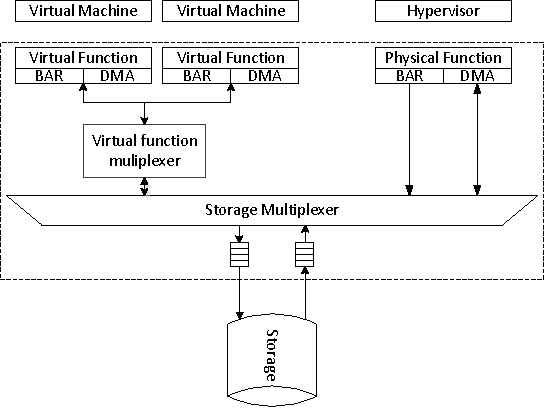
\includegraphics[width=1\columnwidth]{figs/architecture.pdf}
  \caption{An outline of the NeSC architecture. The PF and VFs each have their its set of control registers and request/response queues. The core NeSC microarchitecture multiplexes the activity of the individual VFs.}
  \label{fig:architecture}
\end{figure}
%%%%%%%%%%%%%%%%%%%%

% Add table of the virtual function interface.


% registers only hypervisor can access:
% bus address of extent tree root
% requested write address and size for hypervisor to read when updating tree
%
%registers accessed by virtual machine driver
%lba - start address for upcoming sg list.
%write command list
%read command list
%dma status

As an SR-IOV device, NeSC presents itself as multiple devices on the PCIe interconnect. The architecture must maintain a separate context for each PCIe device (PF and VFs), but a key tenet of the microarchitecture is multiplexing traffic from the different devices.

Figure~\ref{fig:architecture} outlines the core design of the NeSC architecture. For each function (PF and VF alike), NeSC maintains a set of  control registers and request/response queues. All requests sent to the different functions are multiplexed through the address translation and request service units. Similarly, all traffic between the host and the device is multiplexed through a single DMA engine. 

Every request received by the NeSC device is attached with the ID of the NeSC function to which it was sent. This enables the multiplexed facilities to associate requests with a specific function (according to the SR-IOV specification, the ID of the PF is 0). PCIe addressing is hierarchical, and each entity on the interconnect is identified by a triplet: the PCIe \emph{bus ID}, the ID of the device on the bus (\emph{device ID}), and the function inside the device (\emph{function ID}). In PCIe parlance, addresses are referred to as \emph{bus:device:function} triplets or \emph{BDF} for short. Since PCIe addresses of the different NeSC functions share the same bus and device IDs, associating each request with its originating function ID is sufficient for accurate bookkeeping.
The BDF triplet is originated by the PCIe interface of NeSC and is unforgeable by a virtual machine.   



\subsection*{Control registers}
Communication with a PCIe device is handled through \emph{base address registers} (BAR). BARs have a predetermined size, and are mapped to the system's logical address space when the PCIe interconnect is scanned (typically by the system's firmware). Since each BAR is assigned a logical bus address, the hypervisor can map the BARs directly to clients' virtual address spaces, and to its own.

Although NeSC assigns a BAR for each function (physical and virtual alike), the control registers for all functions can be mapped to a single physical structure inside the device.
The PCIe specifications make it possible to define control registers as offsets into a device's BAR. When a certain offset inside a BAR is read from or written to, the PCIe device internally translates the offset to an address in a shared structure.
Since our prototype can support up to 64 VFs (and the additional PF), the NeSC prototype uses a single 130KB SRAM array (2048B per function).

The set of VF-specific control registers are listed as follows (the PCIe specification mandates a number of additional standard control registers, omitted for brevity).
\begin{enumerate}
\item
  \textbf{ExtentTreeRoot} (8B)\quad
  This register contains the base address (in host memory) of the root node of the extent tree associated with a VF. It is set by the hypervisor when a new VF is created. 
%
\item
  \textbf{MissAddress, MissSize} (8B, 4B)\quad
  These two registers are set by NeSC when a translation of a write request sent to the VF misses in the extent tree. After setting these values, NeSC sends an interrupt to the hypervisor so it will allocate additional physical space to the file associated with the VF.
%
\item
  \textbf{RewalkTree} (4B)\quad
  This register is used by the hypervisor to signal NeSC that the physical storage allocation has succeeded. When the hypervisor writes a value of 1 to a VF's RewalkTree register, NeSC reissues the stalled write requests to the extent tree walk unit.
\end{enumerate}

In addition to the NeSC-specific control registers listed above, each VF also exposes a set of registers for controlling a DMA ring buffer~\cite{love10lkd}, which is the de facto standard for communicating with devices. We omit those for brevity.

%%%%%%%%%%%%%%%%%%%%%%%%%%%%%%%%%%%%%%%%%%%%%%%%%%
\subsection{The NeSC virtual function multiplexer}
%%%%%%%%%%%%%%%%%%%%%%%%%%%%%%%%%%%%%%%%%%%%%%%%%%

%%%%%%%%%%%%%%%%%%%%
\begin{figure*}[t]
  \centering
  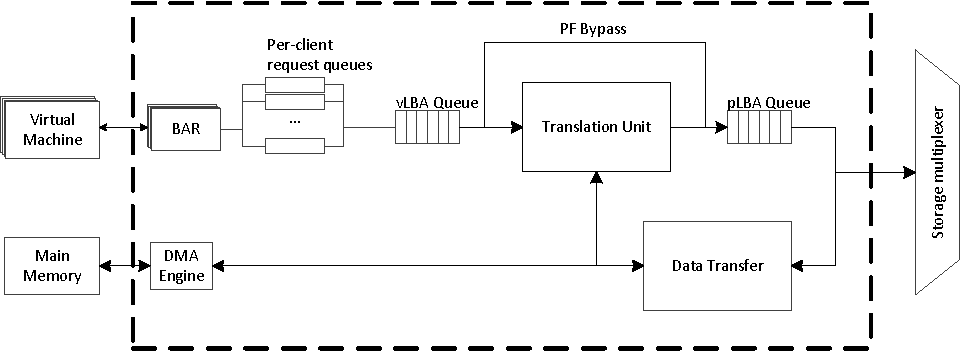
\includegraphics[width=\textwidth]{figs/virtual_function.pdf}
  \caption{High-level view of the NeSC virtual function multiplexer design. The microarchitecture multiplexes requests from the different virtual functions.}
   \label{fig:virtualfunction}
%\end{figure*}
%%%%%%%%%%%%%%%%%%%%

   \vspace*{3ex}
   
%%%%%%%%%%%%%%%%%%%%
%\begin{figure*}[t]
  \centering
  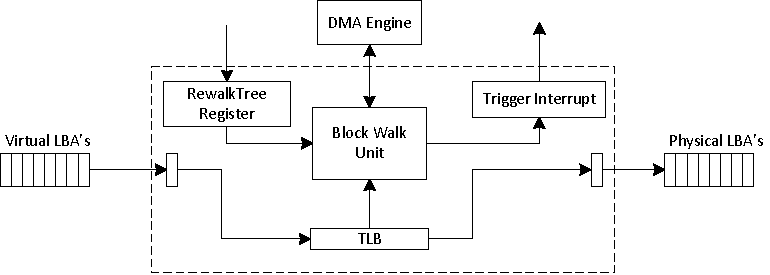
\includegraphics[width=0.9\textwidth]{figs/translation_unit.pdf}
  \caption{The vLBA-to-pLBA translation unit.}
   \label{fig:translation_unit}
\end{figure*}
%%%%%%%%%%%%%%%%%%%%

In this section we describe the implementation of the NeSC virtual function multiplexer, which is depicted in Figure~\ref{fig:virtualfunction}. The main role of the  virtual function multiplexer is to process access requests from the multiple VFs, translate their addresses to physical storage blocks, and respond to the client VM.
%
Access requests are sent by the VM's block driver. The driver typically breaks large requests into a sequence of smaller 4KB requests that match the system's page size. Requests sent from different client VMs are stored in per-client request queues. NeSC dequeues client requests in a round-robin manner in order to prevent client starvation (a full study of client scheduling algorithms and different quality-of-service guarantees is beyond the scope of this paper).

Client requests address their target storage blocks using vLBAs, or logical block addresses as viewed by the virtual device. These addresses must be translated to pLBAs using the per-VF extent tree. The client requests are therefore pushed to a shared vLBA queue for translation, along with the root pointer to their VF's extent tree.

NeSC includes a dedicated \emph{translation unit} (discussed below) that dequeues pending requests from the vLBA queue, translates their vLBAs to pLBAs and pushes the translated requests to a pLBA queue. A \emph{data transfer} unit then manages direct accesses to the persistent storage device. For write requests, the data transfer unit simply writes the data to storage and generates an acknowledge response message that will be sent to the client. For read requests, the data transfer unit reads the target data from the physical storage and prepares a response message. The message is then DMAed to the client VM's destination buffer in host memory.

While we only discuss the processing of client VM requests, NeSC also includes a dedicated out-of-band (OOB) channel to process hypervisor requests sent through the PF. The OOB channel is needed so that VF write requests whose translation is blocked will not block PF requests. The addition of the OOB is, however, simple since PF requests use pLBAs and need not be translated. The OOB channel, therefore, simply adds cuts through to the pLBA queue but does not affect the the address translation unit.

%%%%%%%%%%%%%%%%%%%%%%%%%%%%%%%%%%%%%%%%%%%%%%%%%%
\subsection{The vLBA-to-pLBA translation unit}
%%%%%%%%%%%%%%%%%%%%%%%%%%%%%%%%%%%%%%%%%%%%%%%%%%

The translation unit translates the vLBA addresses used in client VM requests to pLBA addresses, which can be used to access the physical storage. The translation uses the extent tree associated with a request's originating VF.

Figure~\ref{fig:translation_unit} illustrates the translation unit and its components. These include a \emph{block walk unit} that traverses the extent tree and a \emph{translation lookaside buffer} (TLB) that caches recent vLBA mappings. Furthermore, the unit may send interrupts to the hypervisor when a mapping is not found (e.g., when a client VM writes to an unallocated portion of its virtual device), and it is charged with observing the VFs' \emph{RewalkTree} registers through which the hypervisor signals that the mapping was fixed and the extent tree can be re-examined.

%%%%%%%%%%%%%%%%%%%%
\subsubsection*{Block walk unit}
%%%%%%%%%%%%%%%%%%%%
This unit executes the block walk procedure by traversing the extent tree.
When a client VM request arrives at the unit, the root node of the associated extent tree is DMAed and the unit tries to match the vLBA to the offsets listed in the root node's entries (be they node pointers or extent pointers). The matched entry is used as the next node in the traversal, and the process continues recursively until an extent is matched. For read operations, an unmatched vLBA means that the client VM is trying to read from an unmapped file offset (a hole in the file) and zeros must be returned. If a match is not found on a write operation, the unit sets the VF's \emph{MissAddress} and \emph{MissSize} control registers, sends an interrupt to the host, and waits until the hypervisor signals that the missing blocks were allocated (using the \emph{RewalkTree} control register).

The block walk unit is designed for throughput. Since the main performance bottleneck of the unit is the DMA transaction of the next level in the tree, the unit can overlap two translation processes to (almost) hide the DMA latency.

%%%%%%%%%%%%%%%%%%%%
\subsubsection*{Translation lookaside buffer (TLB)}
%%%%%%%%%%%%%%%%%%%%
Given that storage access exhibits spatial locality, and  extents typically span more than one block, the translation unit maintains a small cache of the last 8 extents used in translation. Specifically, this enables the TLB to maintain at least the last mapping for each of the last 8 VFs it serviced.

Before the translation unit begins the block walk, it checks the TLB to see whether the currently translated vLBA matches one of the extents in the TLB. If a match is found, the unit skips the block walk and creates a new pLBA for the output queue.
On a miss, the vLBA will pass to the block walk unit and, after the translation completes, the mapping will be inserted to the TLB (evicting the oldest used extent in the cache).

Finally, the TLB cache must not prevent the hypervisor from executing traditional storage optimizations (e.g., block deduplication). Consequently, NeSC enables the PF (representing the hypervisor) to flush the TLB cache in order to preserve meta-data consistency.

\hide{
%%%%%%%%%%%%%%%%%%%%
\subsubsection*{Data Transfer unit}
%%%%%%%%%%%%%%%%%%%%
This unit interacts with the DMA engine to DMA blocks of storage to and from the storage device.

When a read command is requested by the VM, data blocks are returned by the storage multiplexer to this unit, which in turn will DMA them to the correct address according to the scatter-gather list.

When a write command is requested by the VM, the unit will DMA the blocks from memory and send packets containing the PLBA and the data to the storage multiplexer.
}

In summary, the NeSC implementation effectively balances the need to multiplex different VFs with the application of traditional optimizations such as caching and latency hiding. The following sections describe our evaluation of the proposed NeSC design.

%%%%%%%%%%%%%%%%%%%%%%%%%%%%%%%%%%%%%%%%%%%%%%%%%%%%%%%%%%%%%%%%%%%%%%%%
\section{Methodology}
\label{sec:methodology}
%%%%%%%%%%%%%%%%%%%%%%%%%%%%%%%%%%%%%%%%%%%%%%%%%%%%%%%%%%%%%%%%%%%%%%%%

%%%%%%%%%%%%%%%%%%%%%%%%%%%%%%
\begin{table}[t]
  \centering
  \small
  \begin{tabular}{|p{0.3\columnwidth}|p{0.6\columnwidth}|}
    \hline
    \multicolumn{2}{|c|}{\textbf{Host machine}} \\
    \hline
    Machine model	& Supermicro X9DRG-QF \\
    \hline
    Processor 		& Dual socket Intel(R) Xeon(R) CPU E5-2665 @ 2.40GHz (Sandybridge) \\
    \hline
    Memory 		& 64GB DDR3 1333 MHz \\
    \hline
    Operating system 	& Ubuntu 12.04.5 LTS (kernel 3.5.0) \\
    \hline
    \hline
    \multicolumn{2}{|c|}{\textbf{Virtualized system}} \\
    \hline
    Virtual machine monitor 	& QEMU version 2.2.0 with KVM \\
    \hline
    Guest OS 			& Linux 3.13 \\
    \hline
    Guest RAM 			& 128MB \\
    \hline
    Filesystem on NeSC volume	& ext4 \\
    \hline
    \hline
    \multicolumn{2}{|c|}{\textbf{Prototyping platform}} 	\\
    \hline
    Model		& Xilinx VC707 Evaluation board 	\\
    \hline
    FPGA		& Virtex-7 (XC7VX485T-2FFG1761C) 	\\
    \hline
    RAM			& 1GB DDR3 800MHz 			\\
    \hline
    Host I/O		& PCI Express x8 gen2			\\
    \hline
  \end{tabular}

  \vspace*{1ex}
  \caption{Experimental platform\label{tab:system}}
%  \vspace*{4ex}


  \small
  \begin{tabular}{|p{0.3\columnwidth}|p{0.6\columnwidth}|}
    \hline
    \multicolumn{2}{|c|}{\textbf{Microbenchmark}} \\
    \hline
    GNU dd~\cite{coreutils}	& read/write files using different operational parameters.\\
    \hline
    \hline
    \multicolumn{2}{|c|}{\textbf{Macrobenchmarks}} \\
    \hline
    Sysbench File I/O~\cite{kopytov2004sysbench}
    			& A sequence of random file operations \\
    \hline
    Postmark~\cite{katcher1997postmark}
    			& Mail server simulation \\
    \hline
    MySQL~\cite{mysql}	& Relational database server serving the SysBench OLTP workload  \\
    \hline
    \hline
  \end{tabular}

  \vspace*{1ex}
  \caption{Benchmarks\label{tab:bench}}


\end{table}
%%%%%%%%%%%%%%%%%%%%%%%%%%%%%%


\subsubsection*{\bf Experimental system}
Table~\ref{tab:system} describes our experimental system, which consists of a Supermicro X9DRG-QF server equipped with a Xilinx VC707 evaluation board.

We implemented NeSC using a VC707's Virtex-7 FPGA. Since this revision of the Virtex7 FPGA only supports PCIe Gen2, we had to emulate the self-virtualizing features rather than use the SR-IOV protocol extension. We have emulated the SR-IOV functionalities by dividing the device's memory-mapped BAR to 4KB pages. The first page exports the NeSC PF, and subsequent pages export complete VF interfaces. Upon QEMU startup, the hypervisor maps one of the VF interfaces (offset in the BAR) into the physical address space of the VM. A  multiplexer in the device examines the address to which each PCIe packet (TLP) was sent and queues it to the appropriate VF's command queue. For example, a read TLP that was sent to address 4244 in the NeSC device would have been routed by the multiplexer to offset 128 in the first VF.

Furthermore, since the emulated VFs are not recognized by the IOMMU, VMs cannot DMA data directly to the VC707 board. Instead, the hypervisor allocates trampoline buffers for each VM, and VMs have to copy data to/from the trampoline buffers before/after initiating a DMA operation.

We note that both SR-IOV emulation and trampoline buffers actually impede the performance of NeSC and thereby provide a pessimistic device model. Using a true PCIe gen3 device would improve NeSC's performance.

We further note that we do not emulate a specific access latency technology for the emulated storage device. Instead, we simply use direct DRAM read and write latencies.

We used the QEMU/KVM virtual machine monitor. Since the VC707 board only has 1GB of RAM, we could only emulate 1GB storage on the NeSC device. In order to prevent the entire simulated storage device from being cached in RAM, we limited the VM's RAM to 128MB. We validated that this limitation does not induce swapping in any of the benchmarks.

Finally, in order for NeSC to truly function as a self-virtualizing device, we implemented the VF guest driver, which is a simple block device driver,
and the hypervisor PF driver, which acts as both a block device driver and as the NeSC management driver for creating and deleting VFs.  

\subsubsection*{\bf Benchmarks}
Table~\ref{tab:bench} lists the benchmarks used to evaluate NeSC.
We first evaluated read/write performance metrics (e.g., bandwidth, latency) using the \emph{dd} Unix utility.
In addition, we used a common set of macrobenchmarks that stress the storage system.
All applications used the virtual device through an underlying ext4 filesystem.

\hide{
We evaluated 3 applications and compared their performance speedup when using direct assignment.
All the applications use the virtual device through an underlying EXT4 filesystem.
%
The first application is a MySQL database. We run the OLTP workload using SysBench \cite{kopytov2004sysbench} on the database and measure the TPS. SysBench conduct complex transactional queries along with simple read and write update to the database.
%
The second application is the SysBench file IO benchmark. This benchmark fills the files system with various sized files and randomly reads and writes to and from each of the files. The benchmark measures the total MB/sec.
%
The third application is PostMark~\cite{katcher1997postmark}, which models the workload of an Internet Service Provider under heavy load. PostMark measures TPS. 
}

%%%%%%%%%%%%%%%%%%%%%%%%%%%%%%%%%%%%%%%%%%%%%%%%%%%%%%%%%%%%%%%%%%%%%%%%
\section{Evaluation}
\label{sec:eval}
%%%%%%%%%%%%%%%%%%%%%%%%%%%%%%%%%%%%%%%%%%%%%%%%%%%%%%%%%%%%%%%%%%%%%%%%


%%%%%%%%%%%%%%%%%%%%


%%%%%%%%%%%%%%%%%%%%

%% \begin{table*}[t]
%% \begin{center}
%%   \begin{tabular}{ |l | c | c |c|| c|c|}
%%     \hline
%%     & & & &Direct vs.&Direct vs. \\
%%     Name & virtio & Direct assignment & Emulation & virtio speedup & Emulation speedup\\ \hline \hline
%% %    MySQL - Simple [TPS] & - & - & - \\ \hline
%%     MySQL - Complex [TPS] & 77.6 &	88 & 75.8 & 1.17 & 1.2\\ \hline
%%     Postmark [TPS]&4587.83	&9848.3	&1442.3& 2.1 &6.8\\ \hline
%%     sysbench [Req/s]&214.8&	281.1&	22&1.3&12.7 \\
%%     \hline

%%   \end{tabular}
%%   \caption{Application level benchmarks. Last two columns show the performance speedup of using the direct assignment with NeSC}
%%   \label{macro_bench}

%% \end{center}
%% \end{table*}

%%%%%%%%%%%%%%%%%%%%%%%%%%%%%%%%%%%%%%%%%%%%%%%%%%

%%%%%%%%%%%%%%%%%%%%%%%%%%%%%%%%%%%%%%%%%%%%%%%%%%

This section reports the evaluation results of the NeSC prototype.
We examine the performance benefits of enabling VMs to directly access NeSC, and compare its performance to those of virtio and device emulation.
%% , and raw access to the device by the hypervisor without the virtualization layer.
Our baseline storage device is the NeSC PF, which presents the hypervisor a raw storage device with no file mapping capabilities. The baseline measurement is done by the hypervisor without any virtualization layer.

%%%%%%%%%%%%%%%%%%%%%%%%%%%%%%%%%%%%%%%%%%%%%%%%%%
\subsection{Raw device performance}
%%%%%%%%%%%%%%%%%%%%%%%%%%%%%%%%%%%%%%%%%%%%%%%%%%

We begin by examining the raw device performance observed by the guest VM when accessing a virtual NeSC device. A file on the hypervisor's filesystem is used to create a VF, which is then mapped to the guest VM. These results are compared to mapping the PF itself to the guest VM using either virtio and device emulation. The baseline (marked \emph{Host} in the figures) is the performance observed when the hypervisor directly accesses the PF block device (without virtualization).
In all configurations, we examine the performance of reads and writes to the raw virtual device, without creating a filesystem. 

When a guest accesses the device using virtio or device emulation, each access  request is processed by the guest I/O stack and storage device driver, delivered to the hypervisor, and is then processed by the hypervisor's I/O stack and its own device driver.
When directly assigning a NeSC VF to the guest, the requests pass down the guest I/O stack directly to the device. In contrast, in the baseline evaluation (i.e., \emph{Host} in the figure) the requests pass down the hypervisor I/O stack only.

The performance itself was measured using \emph{dd}~\cite{coreutils} for different block sizes.

%%%%%%%%%%%%%%%%%%%%
\begin{figure}[t]
  \centering
  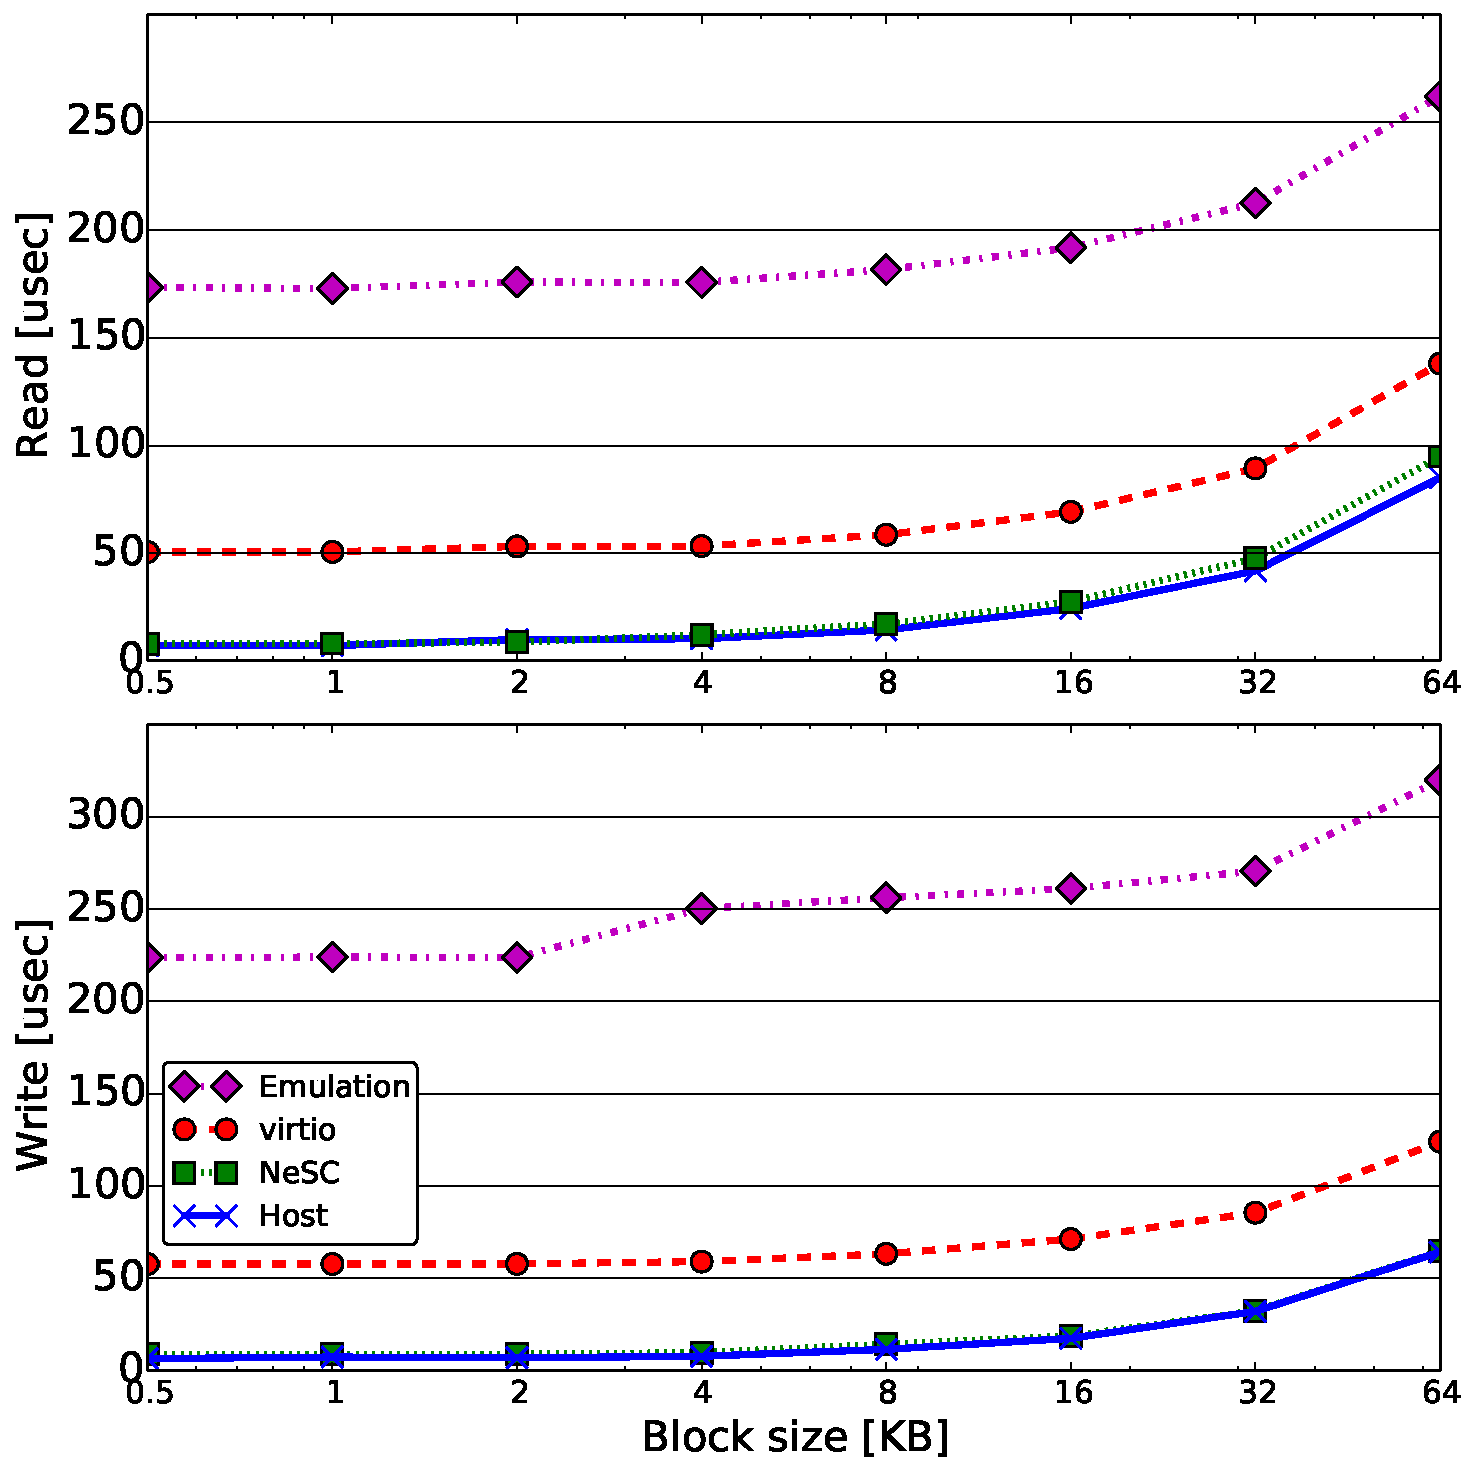
\includegraphics[width=1\columnwidth]{figs/latency_block_size.pdf}
  \caption{Raw access latency observed for read (top) and write (bottom) operations for different block sizes.}
  \label{fig:latency}
\end{figure}
%%%%%%%%%%%%%%%%%%%%

\paragraph{NeSC latency}
Figure~\ref{fig:latency} shows the latency observed for read (top) and write (bottom) operations, using request sizes varying from 512B to 32KB. The figure shows that the latency obtained by NeSC, for both read and write is similar to that obtained by the host when directly accessing the PF. Furthermore, the NeSC latency is  over \speedup{6} faster than virtio and over \speedup{20} faster than device emulation for accesses smaller than 4KB.

%%%%%%%%%%%%%%%%%%%%
\begin{figure}[t]
  \centering
  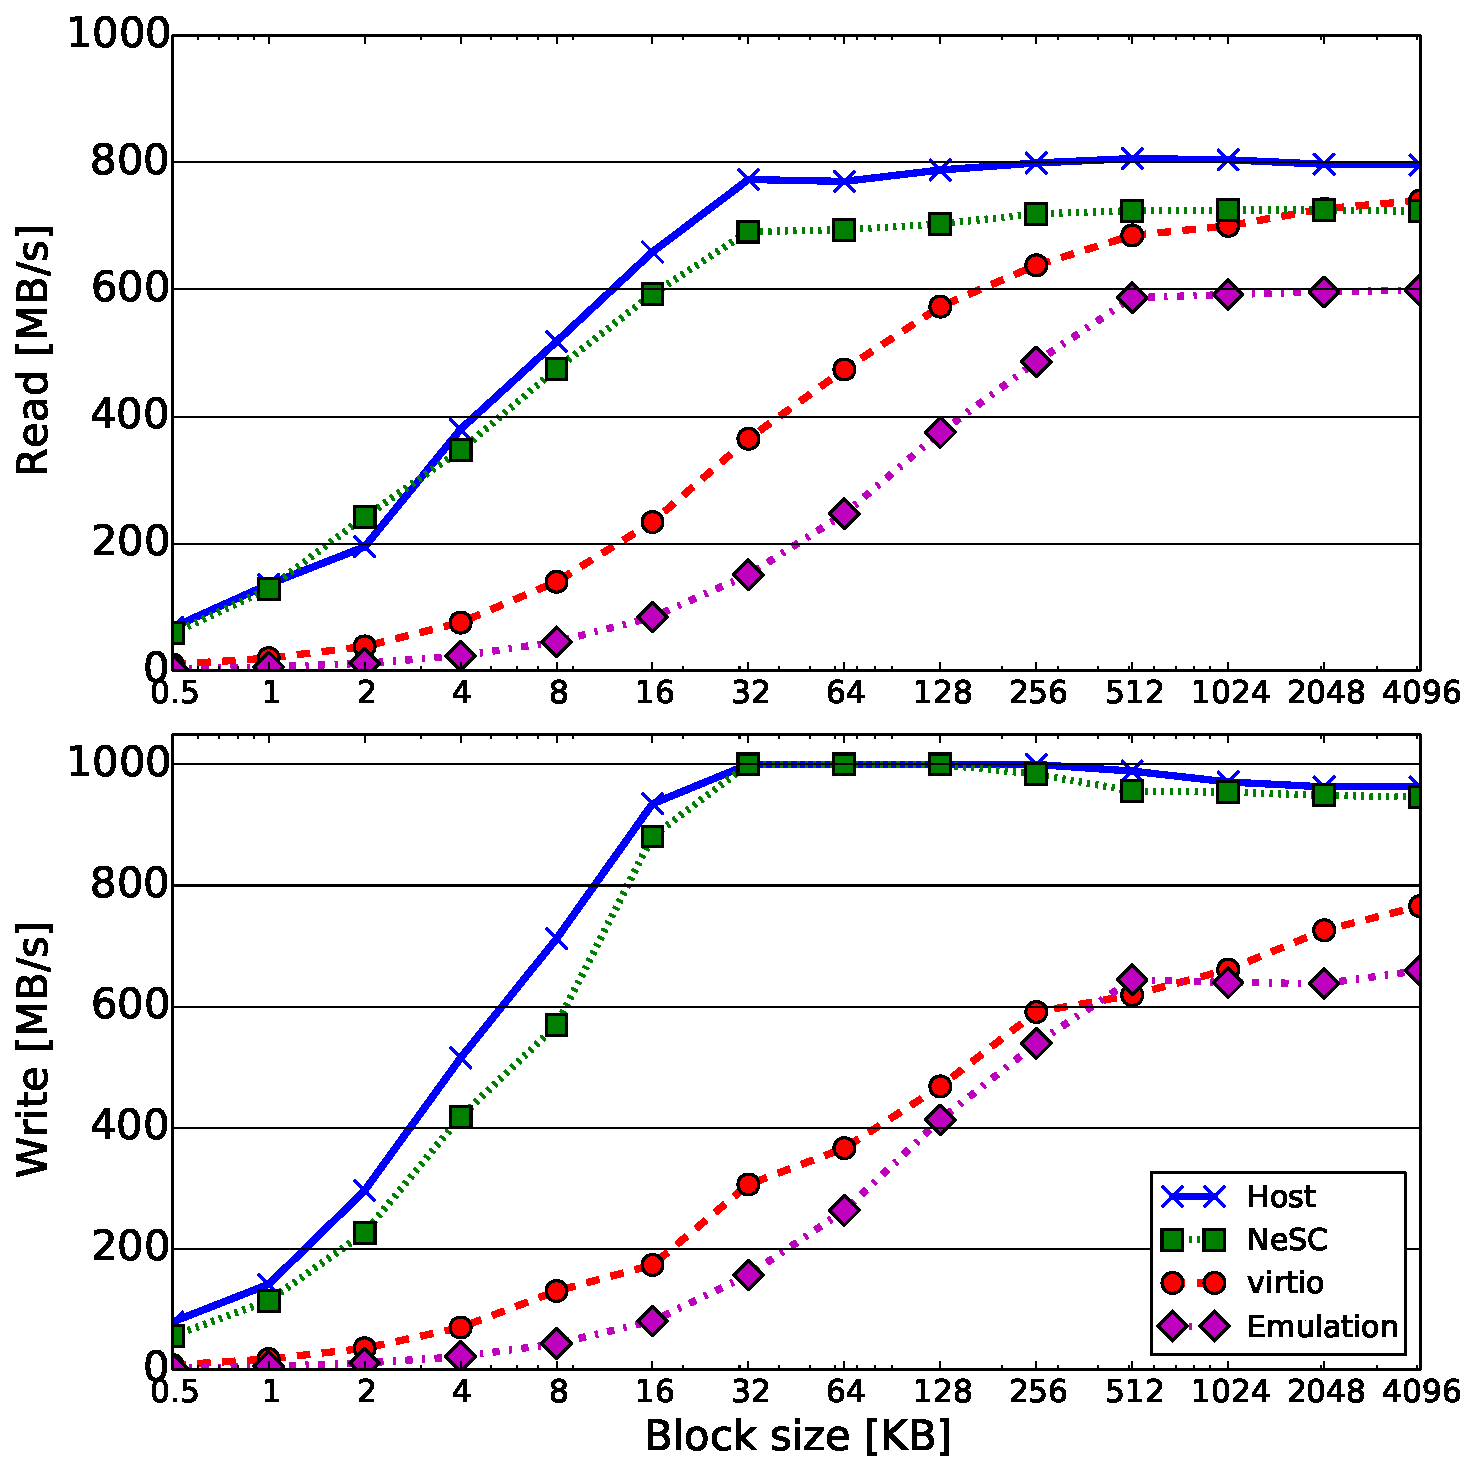
\includegraphics[width=1\columnwidth]{figs/throughput_block_size.pdf}
  \caption{Raw bandwidth observed for read (top) and write (bottom) operations for different block sizes.}
  \label{fig:bw}
\end{figure}
%%%%%%%%%%%%%%%%%%%%

\paragraph{NeSC bandwidth}
Figure~\ref{fig:bw} shows the bandwidth delivered for read (top) and write (bottom) operations, using request sizes varying from 512B to 32KB.

We begin by examining the read bandwidth.
%
The figure shows that for reads smaller than 16KB, NeSC obtained bandwidth close to that of the baseline and outperforms virtio by over \speedup{2.5}.
%
Furthermore, for very large block sizes (over 2MB), the bandwidths delivered by NeSC and virtio converge. This is because such large accesses ameliorate the overheads incurred by VM/hypervisor traps (vmenter/vmexit on Intel platforms).

When examining the write bandwidth, we observe that NeSC delivers performance similar to the baseline for all block sizes. This result is better than that achieved for read bandwidth, for which NeSC is \tilde\percent{10} slower than  the baseline for blocks of size 32KB and larger. Moreover, NeSC's write bandwidth is consistently and substantially better than virtio and emulation, peaking at over \speedup{3} for 32KB block sizes.


%%%%%%%%%%%%%%%%%%%%
\begin{figure}[t]
  \centering
  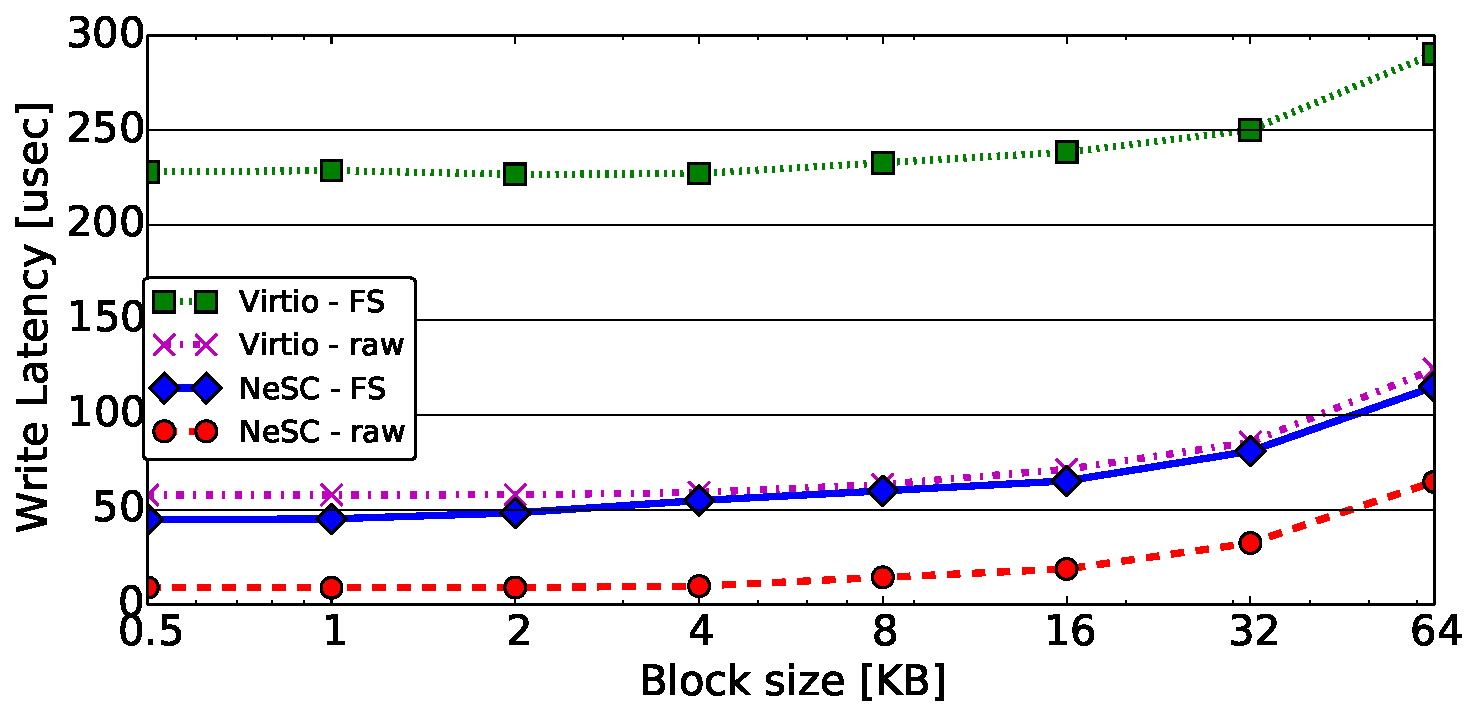
\includegraphics[width=1\columnwidth]{figs/fs_affect.pdf}
  \caption{Filesystem overheads.}
  \label{fig:fs_effect}
\end{figure}
%%%%%%%%%%%%%%%%%%%%

\paragraph{Filesystem overheads}
We next examine the overheads incurred by filesystem translations. To this end, we compare the access latency observed by the guest VM when accessing the raw device with that observed when accessing an ext4 filesystem on the virtual device.

Figure~\ref{fig:fs_effect} shows the write latency when accessing the device with and without a filesystem, for NeSC and virtio virtualization (for brevity, we omit the results obtained using an emulated device since they were much worse than virtio). We only show results for writes because those are more prohibitive for NeSC, since writes may require the VF to request extent allocations from the OS's filesystem.

The figure demonstrates the performance benefits of NeSC. While the filesystem overhead consistently increases NeSC's write latency by \tilde 40\us, the latency provided by NeSC is nevertheless similar to a raw virtio device. Using virtio with a filesystem incurs an extra \tilde 170\us, which is over \speedup{4} slower than NeSC with a filesystem for writes smaller than 8KB.

We note that the similar latencies observed when using a filesystem with NeSC and when using a raw virtio device indicate that NeSC practically eliminates the hypervisor's filesystem overheads.

%%%%%%%%%%%%%%%%%%%%%%%%%%%%%%%%%%%%%%%%%%%%%%%%%%
\subsection{Application performance}
%%%%%%%%%%%%%%%%%%%%%%%%%%%%%%%%%%%%%%%%%%%%%%%%%%

%%%%%%%%%%%%%%%%%%%%
\begin{figure}[t]

  %% \vspace*{-1.5ex}
  \centering
  \subfloat[Applications speedups when using NeSC over device emulation.]{
    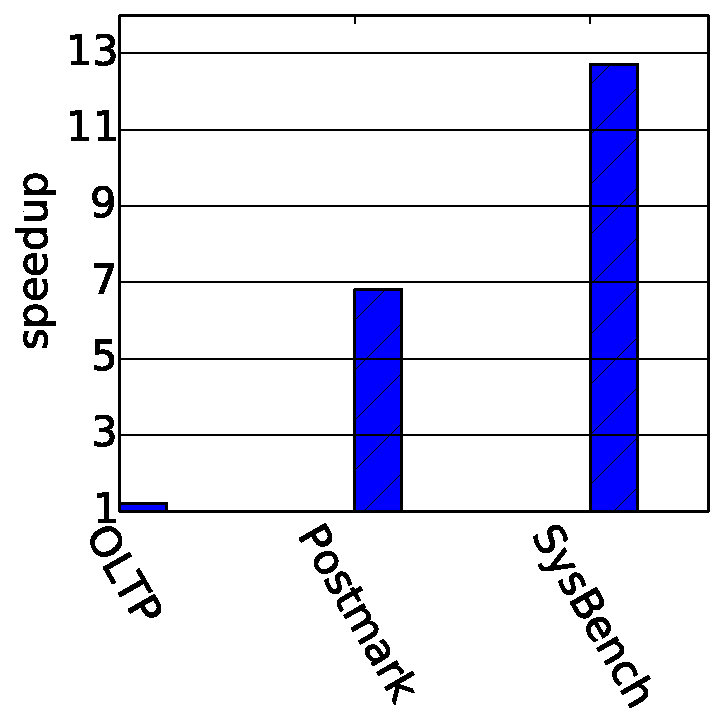
\includegraphics[width=0.48\columnwidth]{figs/application_benchmark_emulation.pdf}
 %   \caption{Read Flow}
    \label{fig:apps_emulation}
  }
  %
  \subfloat[Application speedups when using NeSC over virtio.]{
    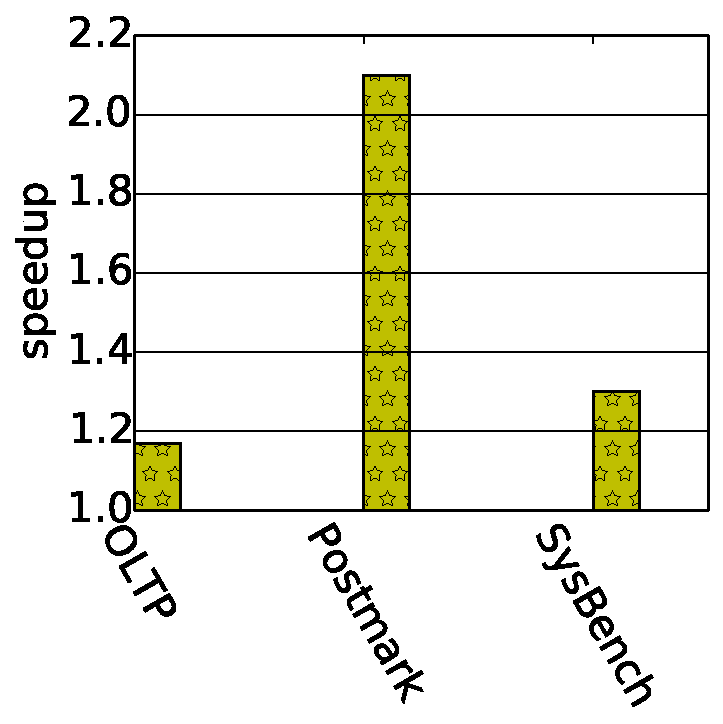
\includegraphics[width=0.48\columnwidth]{figs/application_benchmark_virtio.pdf}
    \label{fig:apps_virtio}
  }
  \caption{Application speedups over other storage virtualization methods.\label{fig:apps}}

    
\end{figure}
%%%%%%%%%%%%%%%%%%%%

We finally examine how the raw performance delivered by NeSC translates to application level speedups. To this end, we compare the performance of the  applications (listed in Figure~\ref{tab:bench}) when running in a guest Linux VM whose storage device is mapped to a NeSC VF, to a virtio device and to a fully emulated device.

The virtual storage device is mapped to the VM in the following manner. The hypervisor creates an ext4 filesystem on the raw device using the NeSC PF. The virtual storage device is stored as an image file (with ext4 filesystem) on  the hypervisor's filesystem, and the hypervisor maps the file to the VM using either of the mapping facilities: virtio, emulation or a NeSC VF.

Figure~\ref{fig:apps} shows the application speedups obtained using a NeSC VF device over device emulation and virtio. For the MySQL OLTP benchmark, the figure shows that mapping the virtual disk using a NeSC virtual device improves performance by \speedup{1.2} over both device emulation (Figure~\ref{fig:apps_emulation}) and virtio (Figure~\ref{fig:apps_virtio}).

The performance improvements provided by NeSC are even more substantial for Postmark and Sysbench File I/O.
Specifically, Postmark enjoys more than \speedup{6} speedup over device emulation and over \speedup{2} over virtio. Sysbench File I/O, on the other hand, enjoys a dramatic \speedup{13} speedup over device emulation, and \speedup{1.3} over virtio.

In summary, the evaluation of the NeSC prototype demonstrates its substantial performance benefits over state-of-the-art storage virtualization methods. The benefits are consistent for both read and write microbenchmarks and for common storage benchmarks.


%%%%%%%%%%%%%%%%%%%%%%%%%%%%%%%%%%%%%%%%%%%%%%%%%%%%%%%%%%%%%%%%%%%%%%%%
\section{Conclusions}
\label{sec:conclusions}
%%%%%%%%%%%%%%%%%%%%%%%%%%%%%%%%%%%%%%%%%%%%%%%%%%%%%%%%%%%%%%%%%%%%%%%%

The emergence of multi-GB/s storage devices has shifted storage virtualization bottlenecks from the storage devices to the software layers. System designers must therefore delegate the virtualization overheads in order to enable virtualized environments to benefit from high-speed storage. 

In this paper we presented the \emph{nested, self-virtualizing storage controller} (NeSC), which enables files stored on the hypervisor-managed filesystem to be directly mapped to guest VMs. NeSC delegates filesystem functionality to the storage device by incorporating mapping facilities that translate file offsets to disk blocks. This enables NeSC to leverage the self-virtualization SR-IOV protocol and thereby expose files as virtual devices on the PCIe interconnect, which can be mapped to\comment{by} guest VMs.

We prototyped NeSC using a Virtex-7 FPGA and evaluated its performance benefits on a real system. Comparing to the leading \emph{virtio} storage virtualization method, we have shown that NeSC practically eliminates the hypervisor's filesystem overheads, as filesystem accesses to a NeSC virtual device incur the same latency as accesses to a raw virtio device.
Furthermore, we have shown that NeSC speeds up common storage benchmarks by \speedup{1.2}--\speedup{2}.

%###############################################################################


%###############################################################################
\hide{
  \section*{Acknowledgments}
  \label{sec:acks}
}

%###############################################################################

%\small
\bibliographystyle{ieeetr}
\bibliography{macros,vdisk}

\end{document}

